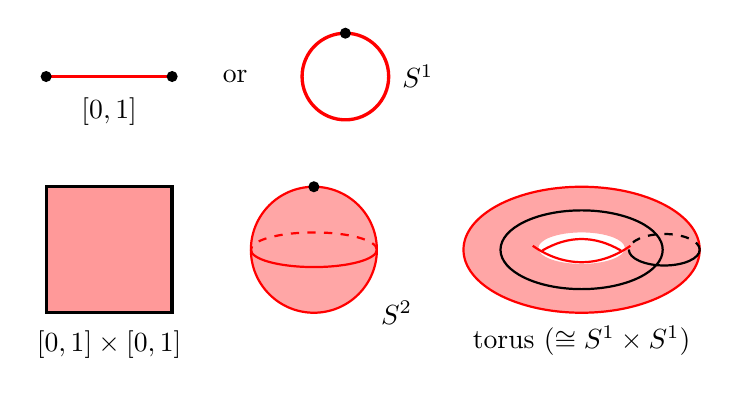
\begin{tikzpicture}
% (0,1) -> [0,1]
\draw[red, very thick] (0,3) -- (1.6,3);
\fill (0,3) circle (2pt); \fill (1.6,3) circle (2pt);
\node[below] at (0.8,2.85) {$[0,1]$};
\node at (2.4,3) {or};
% (0,1) -> S^1
\draw[red, very thick] (3.8,3) circle (0.55);
\fill (3.8,3.55) circle (2pt);
\node[right] at (4.4,3) {$S^1$};
% (0,1)^2 -> square
\fill[red, opacity=0.4] (0,0) rectangle (1.6,1.6);
\draw[very thick] (0,0) rectangle (1.6,1.6);
\node[below] at (0.8,-0.1) {$[0,1]\times[0,1]$};
% sphere
\fill[red, opacity=0.35] (3.4,0.8) circle (0.8);
\draw[red, thick] (3.4,0.8) circle (0.8);
\draw[red, thick] (2.6,0.8) arc[start angle=180, end angle=360, x radius=0.8, y radius=0.22];
\draw[red, thick, dashed] (4.2,0.8) arc[start angle=0, end angle=180, x radius=0.8, y radius=0.22];
\fill (3.4,1.6) circle (2pt);
\node at (4.45,0.0) {$S^2$};
% torus
\begin{scope}[shift={(6.8,0.8)}]
\fill[red, opacity=0.35, even odd rule] (0,0) ellipse (1.5 and 0.8) (0,0.02) ellipse (0.55 and 0.2);
\draw[red, thick] (0,0) ellipse (1.5 and 0.8);
\draw[red, thick] (-0.62,0.05) to[bend right=35] (0.62,0.05);
\draw[red, thick] (-0.5,-0.01) to[bend left=30] (0.5,-0.01);
\draw[thick] (0,0) ellipse (1.03 and 0.5);
\draw[thick] (0.6,0) arc[start angle=180, end angle=360, x radius=0.45, y radius=0.2];
\draw[thick, dashed] (1.5,0) arc[start angle=0, end angle=180, x radius=0.45, y radius=0.2];
\node[below] at (0,-0.85) {torus ($\cong S^1\times S^1$)};
\end{scope}
\end{tikzpicture}
